\documentclass[11pt]{article}

\usepackage[margin=1.7cm]{geometry}
\usepackage{amsmath}
\usepackage{amssymb}
\usepackage{enumitem}
\usepackage{titlesec}
\usepackage{xcolor}
\usepackage{fancyhdr}
\usepackage{tikz}
\usetikzlibrary{arrows.meta}
\usepackage{pgfplots}
\usepackage{multicol}
\usepackage{array}
\pgfplotsset{compat=1.18}

\titleformat{\section}{\large\bfseries}{\thesection}{0.6em}{}
\titlespacing{\section}{0pt}{1.1em}{0.5em}

\pagestyle{fancy}
\fancyhf{}
\fancyhead[L]{Year 9 Algebra Revision --- Basics}
\fancyhead[R]{Name: \makebox[4cm]{\hrulefill}}
\fancyfoot[C]{\thepage}
\renewcommand{\headrulewidth}{0.4pt}

\newcommand{\ans}{\hrulefill}
\setlist[enumerate,1]{leftmargin=1.4em, itemsep=0.5em, topsep=0.2em}
\setlength{\columnsep}{1.1cm}
\setlength{\columnseprule}{0.4pt}

% dot + coordinate label
\newcommand{\markpt}[3]{\filldraw (axis cs:#1,#2) circle (1.5pt); \node[#3, font=\small] at (axis cs:#1,#2) {$(#1,#2)$};}
% dot only
\newcommand{\dotpt}[2]{\filldraw (axis cs:#1,#2) circle (1.5pt);}

% \gridaxis{xmin}{xmax}{ymin}{ymax}{tick distance}
\newcommand{\gridaxis}[5]{%
  \begin{axis}[
    width=7cm, height=6.4cm,
    xmin=#1, xmax=#2, ymin=#3, ymax=#4,
    grid=both, grid style={line width=.1pt, draw=gray!35},
    axis lines=middle,
    xlabel={$x$}, ylabel={$y$},
    xtick distance=#5, ytick distance=#5,
    tick label style={font=\tiny},
    label style={font=\small},
    xlabel style={at={(axis description cs:1,0)}, anchor=north west},
    ylabel style={at={(axis description cs:0,1)}, anchor=south east},
    axis line style={-{Latex[length=1.8mm]}},
  ]
}

\begin{document}

\begin{center}
  {\Large\bfseries Year 9 Algebra Revision --- Basics}
\end{center}
\vspace{0.3em}
\noindent\textit{Straightforward practice of each skill on its own --- no multi-step problems yet.}

\vspace{0.4em}
\section{Simplifying Expressions}

\begin{multicols}{2}
\subsection*{Adding and subtracting like terms}
\begin{enumerate}
  \item $3x + 5x$ \ans
  \item $9y - 4y$ \ans
  \item $4a + 3a - 2a$ \ans
  \item $5x + 2y + 2x - y$ \ans
\end{enumerate}

\subsection*{Multiplying and dividing}
\begin{enumerate}[resume]
  \item $3 \times 4x$ \ans
  \item $(-2) \times 5a$ \ans
  \item $12x \div 4$ \ans
  \item $20y \div 5$ \ans
\end{enumerate}
\end{multicols}

\section{Solving Equations}

\begin{multicols}{2}
\subsection*{One-step equations}
\begin{enumerate}
  \item $x + 7 = 12$ \ans
  \item $x - 5 = 9$ \ans
  \item $4x = 24$ \ans
\end{enumerate}

\subsection*{Two-step equations}
\begin{enumerate}[resume]
  \item $2x + 3 = 11$ \ans
  \item $3x - 4 = 11$ \ans
  \item $\dfrac{x}{2} + 1 = 5$ \ans
\end{enumerate}

\subsection*{Multi-step equations}
\begin{enumerate}[resume]
  \item $2(x + 3) = 16$ \ans
  \item $3x + 2x - 1 = 14$ \ans
  \item $5x - 3 - x = 9$ \ans
\end{enumerate}

\subsection*{Variables on both sides}
\begin{enumerate}[resume]
  \item $3x + 2 = x + 10$ \ans
  \item $5x - 1 = 2x + 8$ \ans
  \item $4x + 3 = 2x + 11$ \ans
\end{enumerate}
\end{multicols}

\newpage
\section{Tables of Values}
\noindent Complete each table using the given rule.

\begin{center}
\begin{tabular}{|c|c|c|c|c|c|c|}
\hline
\multicolumn{7}{|l|}{$y = x + 3$} \\\hline
$x$ & $-2$ & $-1$ & $0$ & $1$ & $2$ & $3$ \\\hline
$y$ & & & & & & \\\hline
\end{tabular}

\vspace{1em}

\begin{tabular}{|c|c|c|c|c|c|c|}
\hline
\multicolumn{7}{|l|}{$y = 2x - 1$} \\\hline
$x$ & $-2$ & $-1$ & $0$ & $1$ & $2$ & $3$ \\\hline
$y$ & & & & & & \\\hline
\end{tabular}
\end{center}

\vspace{1em}
\section{Plotting Points}
\noindent Plot and label each of these points on the Cartesian plane below.
\[
  (2,3) \quad (-3,1) \quad (0,-4) \quad (-2,-2) \quad (4,0) \quad (-4,4) \quad (1,-3)
\]

\begin{center}
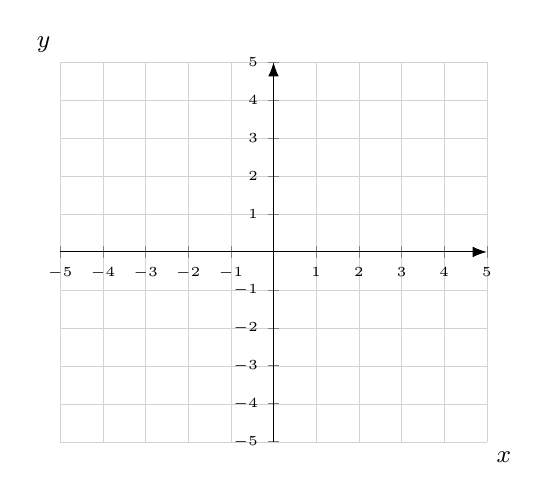
\begin{tikzpicture}
\gridaxis{-5}{5}{-5}{5}{1}
\end{axis}
\end{tikzpicture}
\end{center}

\newpage
\section{Drawing a Line from an Equation}
\noindent For each equation: complete the table, plot the points on the grid, then draw a straight line through them.

\begin{center}
\begin{minipage}{0.48\linewidth}
\centering
$y = x + 1$

\vspace{0.5em}
\begin{tabular}{|c|c|c|c|c|c|}
\hline
$x$ & $-2$ & $-1$ & $0$ & $1$ & $2$ \\\hline
$y$ & & & & & \\\hline
\end{tabular}

\vspace{0.8em}
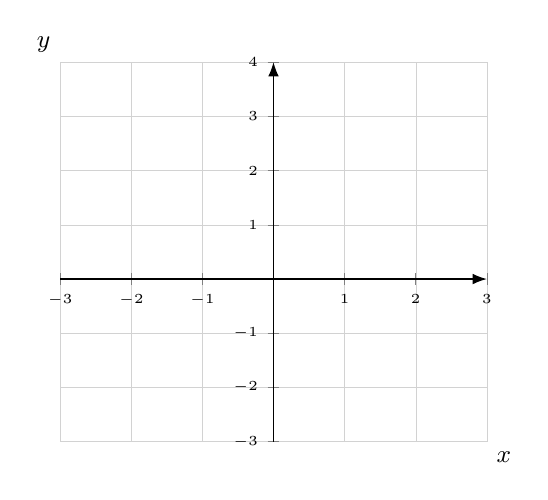
\begin{tikzpicture}
\gridaxis{-3}{3}{-3}{4}{1}
\end{axis}
\end{tikzpicture}
\end{minipage}
\hfill
\begin{minipage}{0.48\linewidth}
\centering
$y = -2x + 3$

\vspace{0.5em}
\begin{tabular}{|c|c|c|c|c|c|}
\hline
$x$ & $-1$ & $0$ & $1$ & $2$ & $3$ \\\hline
$y$ & & & & & \\\hline
\end{tabular}

\vspace{0.8em}
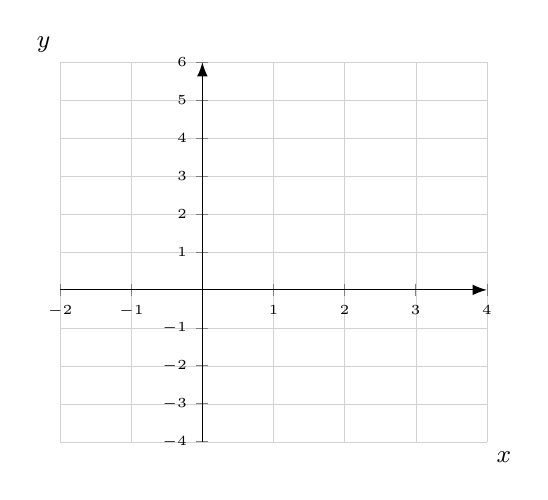
\begin{tikzpicture}
\gridaxis{-2}{4}{-4}{6}{1}
\end{axis}
\end{tikzpicture}
\end{minipage}
\end{center}

\newpage
\section{Reading a Line: $y$-intercept, Gradient, Equation}
\noindent For each graph, find: (a) the $y$-intercept, (b) the gradient (using the triangle shown), and (c) the equation of the line in the form $y = mx + c$.

\begin{center}
\begin{minipage}{0.48\linewidth}
\centering
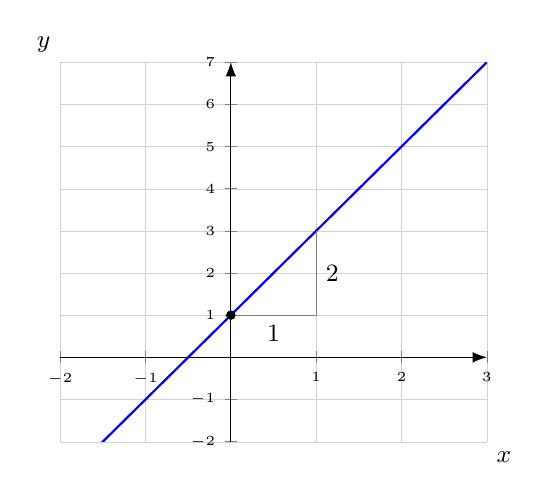
\begin{tikzpicture}
\gridaxis{-2}{3}{-2}{7}{1}
\addplot[domain=-2:3, samples=2, thick, blue] {2*x+1};
\draw[gray] (axis cs:0,1) -- (axis cs:1,1) -- (axis cs:1,3);
\node[below, font=\small] at (axis cs:0.5,1) {$1$};
\node[right, font=\small] at (axis cs:1,2) {$2$};
\dotpt{0}{1}
\end{axis}
\end{tikzpicture}

\vspace{0.3em}
(a) $y$-intercept: \ans \\[0.5em]
(b) Gradient: \ans \\[0.5em]
(c) Equation: \ans
\end{minipage}
\hfill
\begin{minipage}{0.48\linewidth}
\centering
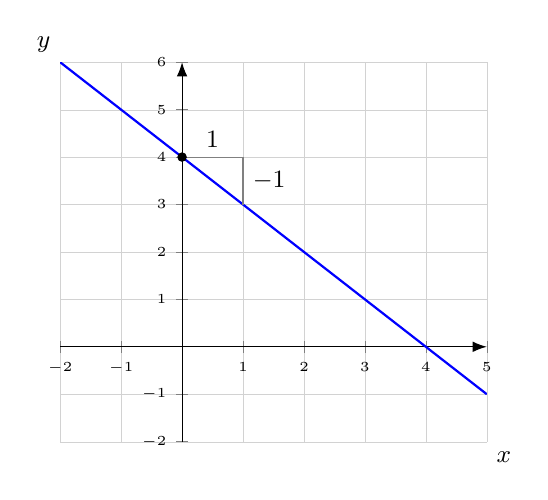
\begin{tikzpicture}
\gridaxis{-2}{5}{-2}{6}{1}
\addplot[domain=-2:5, samples=2, thick, blue] {-x+4};
\draw[gray] (axis cs:0,4) -- (axis cs:1,4) -- (axis cs:1,3);
\node[above, font=\small] at (axis cs:0.5,4) {$1$};
\node[right, font=\small] at (axis cs:1,3.5) {$-1$};
\dotpt{0}{4}
\end{axis}
\end{tikzpicture}

\vspace{0.3em}
(a) $y$-intercept: \ans \\[0.5em]
(b) Gradient: \ans \\[0.5em]
(c) Equation: \ans
\end{minipage}
\end{center}

\vspace{1em}
\section{Reading a Table: $y$-intercept, Gradient, Equation}
\noindent For each table, find: (a) the $y$-intercept, (b) the gradient, and (c) the equation of the line in the form $y = mx + c$.

\begin{center}
\begin{minipage}{0.48\linewidth}
\centering
\begin{tabular}{|c|c|c|c|c|}
\hline
$x$ & $0$ & $1$ & $2$ & $3$ \\\hline
$y$ & $2$ & $5$ & $8$ & $11$ \\\hline
\end{tabular}

\vspace{0.6em}
(a) $y$-intercept: \ans \\[0.5em]
(b) Gradient: \ans \\[0.5em]
(c) Equation: \ans
\end{minipage}
\hfill
\begin{minipage}{0.48\linewidth}
\centering
\begin{tabular}{|c|c|c|c|c|}
\hline
$x$ & $0$ & $1$ & $2$ & $3$ \\\hline
$y$ & $5$ & $3$ & $1$ & $-1$ \\\hline
\end{tabular}

\vspace{0.6em}
(a) $y$-intercept: \ans \\[0.5em]
(b) Gradient: \ans \\[0.5em]
(c) Equation: \ans
\end{minipage}
\end{center}

\end{document}
